\documentclass[bwprint]{gmcmthesis}
\usepackage{amsmath}
\numberwithin{figure}{section}
\usepackage{hyperref}
\renewcommand{\thefigure}{\arabic{section}-\arabic{figure}} 
\newcommand{\upcite}[1]{\textsuperscript{\textsuperscript{\cite{#1}}}} 
% \documentclass[withoutpreface,bwprint]{cumcmthesis}
% 去掉封面与编号页
\hypersetup{
    colorlinks=true,      
    urlcolor=cyan,
    pdftitle={Overleaf Example},
    pdfpagemode=FullScreen,
    }
\title{荷兰2050年碳中和的可能性}
\baominghao{T1-0275} %参赛队号
\tihao{2022-T1-0275\_kGkpjeMr} %论文编号
\schoolname{未来精工技术学院}%学校名称
\membera{马煜} %队员A
\memberb{艾煜明} %队员B
\memberc{张佳馨} %队员C
\memberd{曹鹏}%指导教师
\begin{document}
\maketitle
\begin{abstract}
	现阶段世界大部分国家和国际组织都提出了碳中和计划。为了讨论各个国家
	碳中和计划能否实现,以及如何实现,
	我们需要建立快捷方便的模型来评估和规划碳中和计划,从而更好的缓解人类发展和环境的冲突。
	本文以荷兰为示例建立模型。
	
	针对第一问,通过广泛收集数据,以一定的条件筛选数据,
	再对其应用不同的模型进行分析,建立了以灰色预测模型GM(1,1)为基础的
	预测模型,成功的对以荷兰为例的碳中和指标进行了预测。
	
	针对第二问,基于2050年实现零排放的气候目标,参考政府报告和目前主流碳吸收手段的基本参数,分析给出相对可行的碳吸收建设方案。围绕碳捕集、森林和海洋碳吸收为主要途径,在2050年基本实现年吸收量超过68Mt。

	针对第三问,我们结合第一问中的碳排放预测结果和第二问提出的碳吸收能以建设意见,考虑经济等方面成本,
	认为荷兰现有资源可以支持上述预测结果,使之成为现实。

	经过我们团队的建模分析,我们认为荷兰能够在2050年完成碳中和目标。该国碳中和路径规划对欧盟其他国家乃至世界各国都有较强的借鉴意义。

	\keywords{零排放\quad 碳中和\quad 荷兰\quad 灰色预测模型(Gray Forecast Model)\quad }
\end{abstract}

%\pagestyle{plain}

%目录
\tableofcontents
\newpage
\section{问题背景及重述}
\subsection{背景}
在经济飞速发展和人口急剧增长以及科技革新的21世纪初,世界人民已经迈向了新的生活时代,
观念也有了长足的进步。人类对于环境的影响日益增强,对于环境保护的理念理解也在不断进步。
世界能源转型是实现国家和区域能源安全的必然选择,是推动世界经济发展和经济增长的新动力,
是重塑世界政治格局的新力量,是切实履行《巴黎协定》要求、实现能源利用"碳中和"目标、
应对全球气候变化的有效举措。\upcite{bib:one} 所谓碳中和就是在进入大气的温室
气体排放和吸收的汇之间达到平衡。因为前人为温室气体排放的绝大部分是 $CO_{2}$,
因此在各国提出的中和或净零排放目标被代指为碳中和。\upcite{meaning}

相关报道表明,碳中和正在成为全球气候行动关注的重要内容,
对于推进全球应对气候变化具有积极意义。而欧盟等
发达国家 / 地区目前在碳中和行动中起到关键引领作用。\upcite{bib:3}
因此我们选取欧盟中发展水平适中,综合国力和科技经济发展水平
较为平均的荷兰作为分析对象。荷兰在2020年GDP为$912.2 \text{billion USD}$,目前排世界第14位;根据荷兰统计局
2016年的数据,荷兰排欧盟第6位,较能代表欧洲发展的平均水平。且荷兰为西欧代表国家,其气候等地理特征能较好的
贴合欧盟大部分国家。荷兰已经有计划的实时他们自己的碳排放政策。

借由新冠肺炎(COVID-19)疫情大流行造成各国经济萎缩,
各国政府正在积极制定经济复苏政策。
恰好可以采用低碳复苏的方式,可以通过加大可再生能源投资等公
共支出来实现向可持续、低碳经济的长期转型。

在这样的国际大背景下,为了讨论各个国家碳中和计划能否实现,以及
如何实现,我们需要建立快捷方便的模型来评估和规划碳中和计划,从而更好的缓解人类
发展和环境的冲突就刻不容缓。
\subsection{问题重述}
\begin{itemize}
	\item 选取现有合适预测模型进行评估,考虑不同维度,不同历史时间段,
	对发电量和发电所需要的碳排放量进行预测,并对该模型的结果进行精度分析。
	\item 根据相对应国家地理环境特征和技术发展,选取可行的碳吸收手
	段并加权计算对应碳吸收量
	\item 根据前两步结果,计算方案成本和该国实际发展水平的关系,
	评估可行性
\end{itemize}

\section{模型假设}
\begin{enumerate}
\item 我们认为未来发展不受战争等突发因素影响,发展符合客观发展规律。\upcite{bib:4}
\item 我们认为未来35年不会出现颠覆性的能源技术。
\item 认为该国家会全力执行现有的碳中和战略。\label{jiashe}
\item 认为可再生能源产生的碳排放量相比于传统能源(如天然气,煤炭,原油)产生的碳排放量可以忽略不计。\upcite{kezaishengnengyuan}
\item 认为可再生能源发电量在政策主导下短期内(25年内)能维持指数增长。
\item 认为数据源准确可信。
\end{enumerate}

\section{符号说明}
\begin{itemize}
	\item 字母符号上带有“\^{}”的表示估计值或拟合值,如$\hat{a}$表示发展灰数的拟合值。
\end{itemize}

\section{问题的分析和模型的建立}
\subsection{预测碳中和目标年份所需发电量和生产电力产生的碳排放量}
\subsubsection{问题分析}
%先分析问题本身
我们首先对概念本身及数据的收集结合题目进行了分析。

对于碳中和这个概念,根据相关资料查询,气候中和并不必然要求温室气体净零排放。
对于 $CH_4$ 等短寿命温
室气体而言,稳定的短寿命温室气体
排放并不会导致新的气候影响,因此气候中和只
要求短寿命温室气体排放达到稳定而不必要求其
达到零排放。\upcite{meaning}

根据现有数据来看,立法或出台协定或政策的国家家并
未严格遵循 IPCC 的定义,造成了气体覆盖范围不明晰的情况。于是我们选择公认的$CO_{2}$作为指标,忽略其他温室气体如
$NO_{2}\text{和}CH_{4}$的影响。\upcite{meaning}

为了综合考虑各方的数据来源,我们认为可以从该国政府网站、能源相关国际组织(如BP energy partners,世界银行) 查找有关数据。
问题一要求我们首先从各种数据来源收集可靠数据,考虑到各个数据来源的数据规模,
时间跨度,数据维度均有不同程度的差异。为保证建立模型的数据精确可靠,需要进行简单筛选。
我们采取检索数据源可信度,手动对比数据、剔除明显异常和数据量过少数据源等方式,
提高数据可信度。

为了对数据趋势和数量级有初步认识,可以将提取完的数据将数据各个维度与时间关联作图。帮助我们把握数据的结构,从而构建相应的模型。

考虑各个国家的发展水平和国情以及地理环境的差异,使得建立一个通用的模型有一定的难度。
但若能选择一个能以各个国家历史能源数据建立的模型,能在数据中体现出上述因素对碳中和的影响。便能更加体现我们模型的普适性。

为了使我们的模型能更好的匹配欧盟国家,我们结合国家发展的平均水平选择了“风车之国”荷兰来建立和评估我们的模型。
我们最初打算选择使用灰色预测模型GM(1,1)
来预测总发电量和生产这些电力所需要的总发电量。之所以首先灰色预测模型,
是考虑到灰色系统理论已经成功的用于工程控制、经济管理、未来学研究、
生态系统及复杂多变的农业系统中,并取得了一定的成就和认可。
结合我们能找到的公开数据,以及对近些年世界政治经济快速变化,
发展的理解,我们认为手中得到的数据量较少且分类粗糙,不适合其他以回归分析为代表的常用的预测方法。
灰度预测模型恰好是一个通过少量的、不完全的信息建立数学模型的预测方法。
在样本量较小的时候,所需信息量少,运算方便,建模精度高,能快速评估各国的碳中和战略可行性。

在进行了上述分析之后,我们在建模操作中发现问题解决问题,过程如下:
\subsubsection{模型建立与求解}
\begin{itemize}
	\item \textbf{总发电量预测}
\end{itemize}

\begin{itemize}
	\item 模型的准备
\end{itemize}

荷兰1985年至2020年的年度总发电量数据从\href{http://www.bp.com/statisticalreview}{BP energy partners}中得到,对荷兰1985年至2020年总发电量数据处理观察,容易得出荷兰年总发电量增长稳定,波动较小,预计至2050年,荷兰在不发生重大变故的情况下,其所需电量与总发电量会稳步提升,这是对荷兰年度总发电量的整体预测分析。而对荷兰总发电量按发电来源分解来看,通过对原始数据的直观构图观察,初步得到各种发电来源发电量随年份的变化规律。并且通过对比,发现荷兰在本世纪初至今,发电的主要来源都是天然气和煤炭,尽管各年天然气和煤炭发电量变化较显著,但二者发电量之和趋于平稳;2010年,荷兰风力发电量开始以指数形势增长,2015年,荷兰太阳能光伏发电和生物燃烧发电也显著提高。考虑历史、技术要求等因素,在未来30年内,荷兰天然气和煤炭发电量将会显著减少,取而代之的是目前供给发电以指数形式增长的可再生能源,包括风力发电,生物质能发电,太阳能发电,水力发电。再在荷兰政府颁布的相关政策文件的基础上,可以合理外推得出,荷兰未来发电方式会从以煤炭原油天然气等传统能源向以可再生能源转变。(参见图\ref{fig_1}图\ref{fig_2})

\begin{figure}[!h]
	\centering
	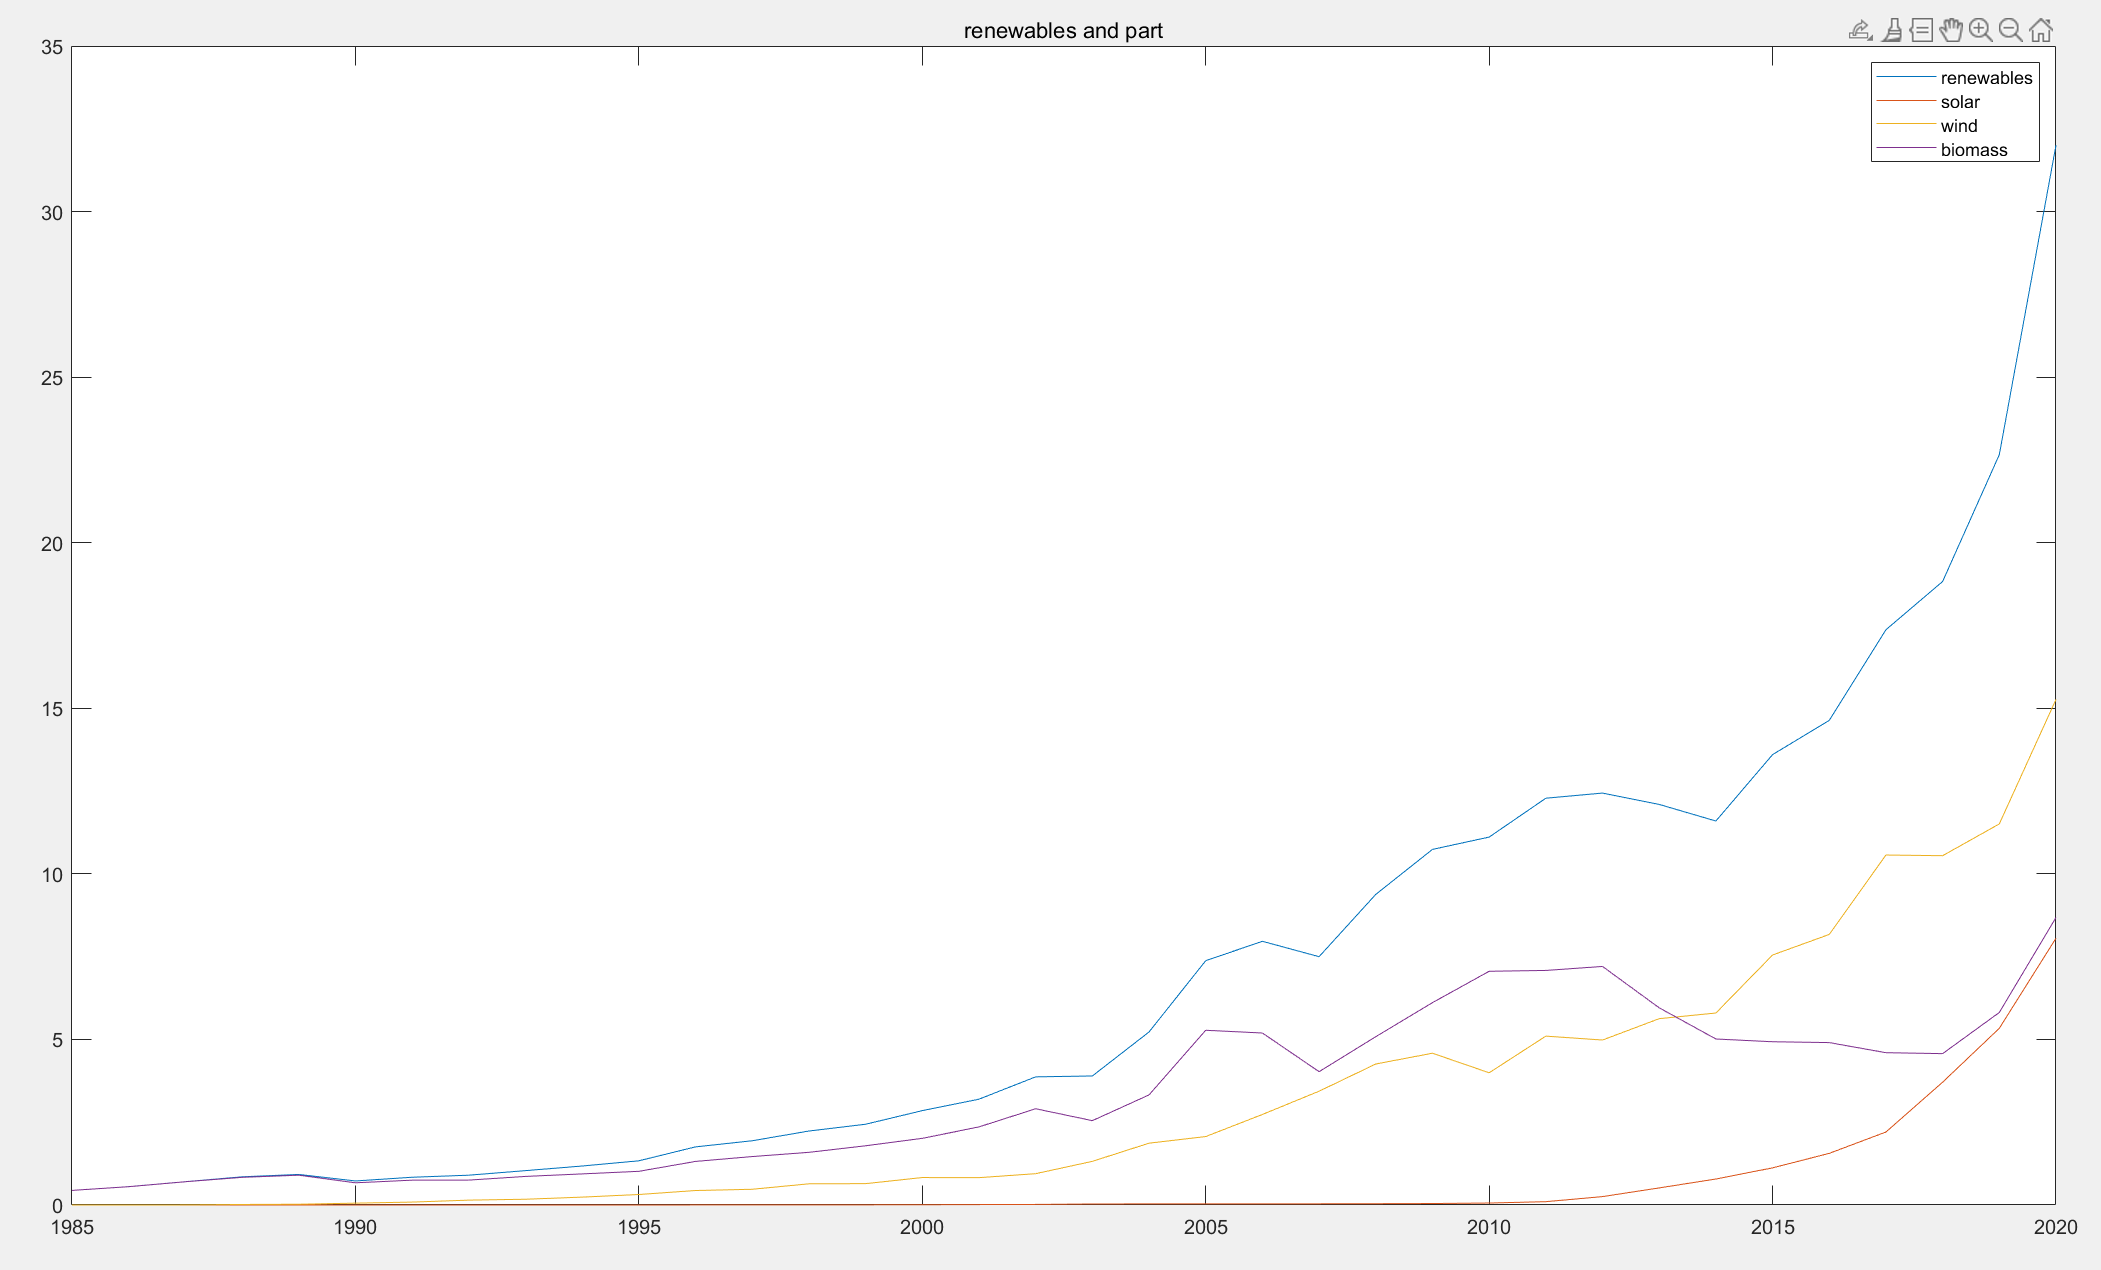
\includegraphics[width=.7\textwidth]{renewables and part.png}
	\caption{renewables and part}
	\label{fig_1}
\end{figure}

\begin{figure}[!h]
	\centering
	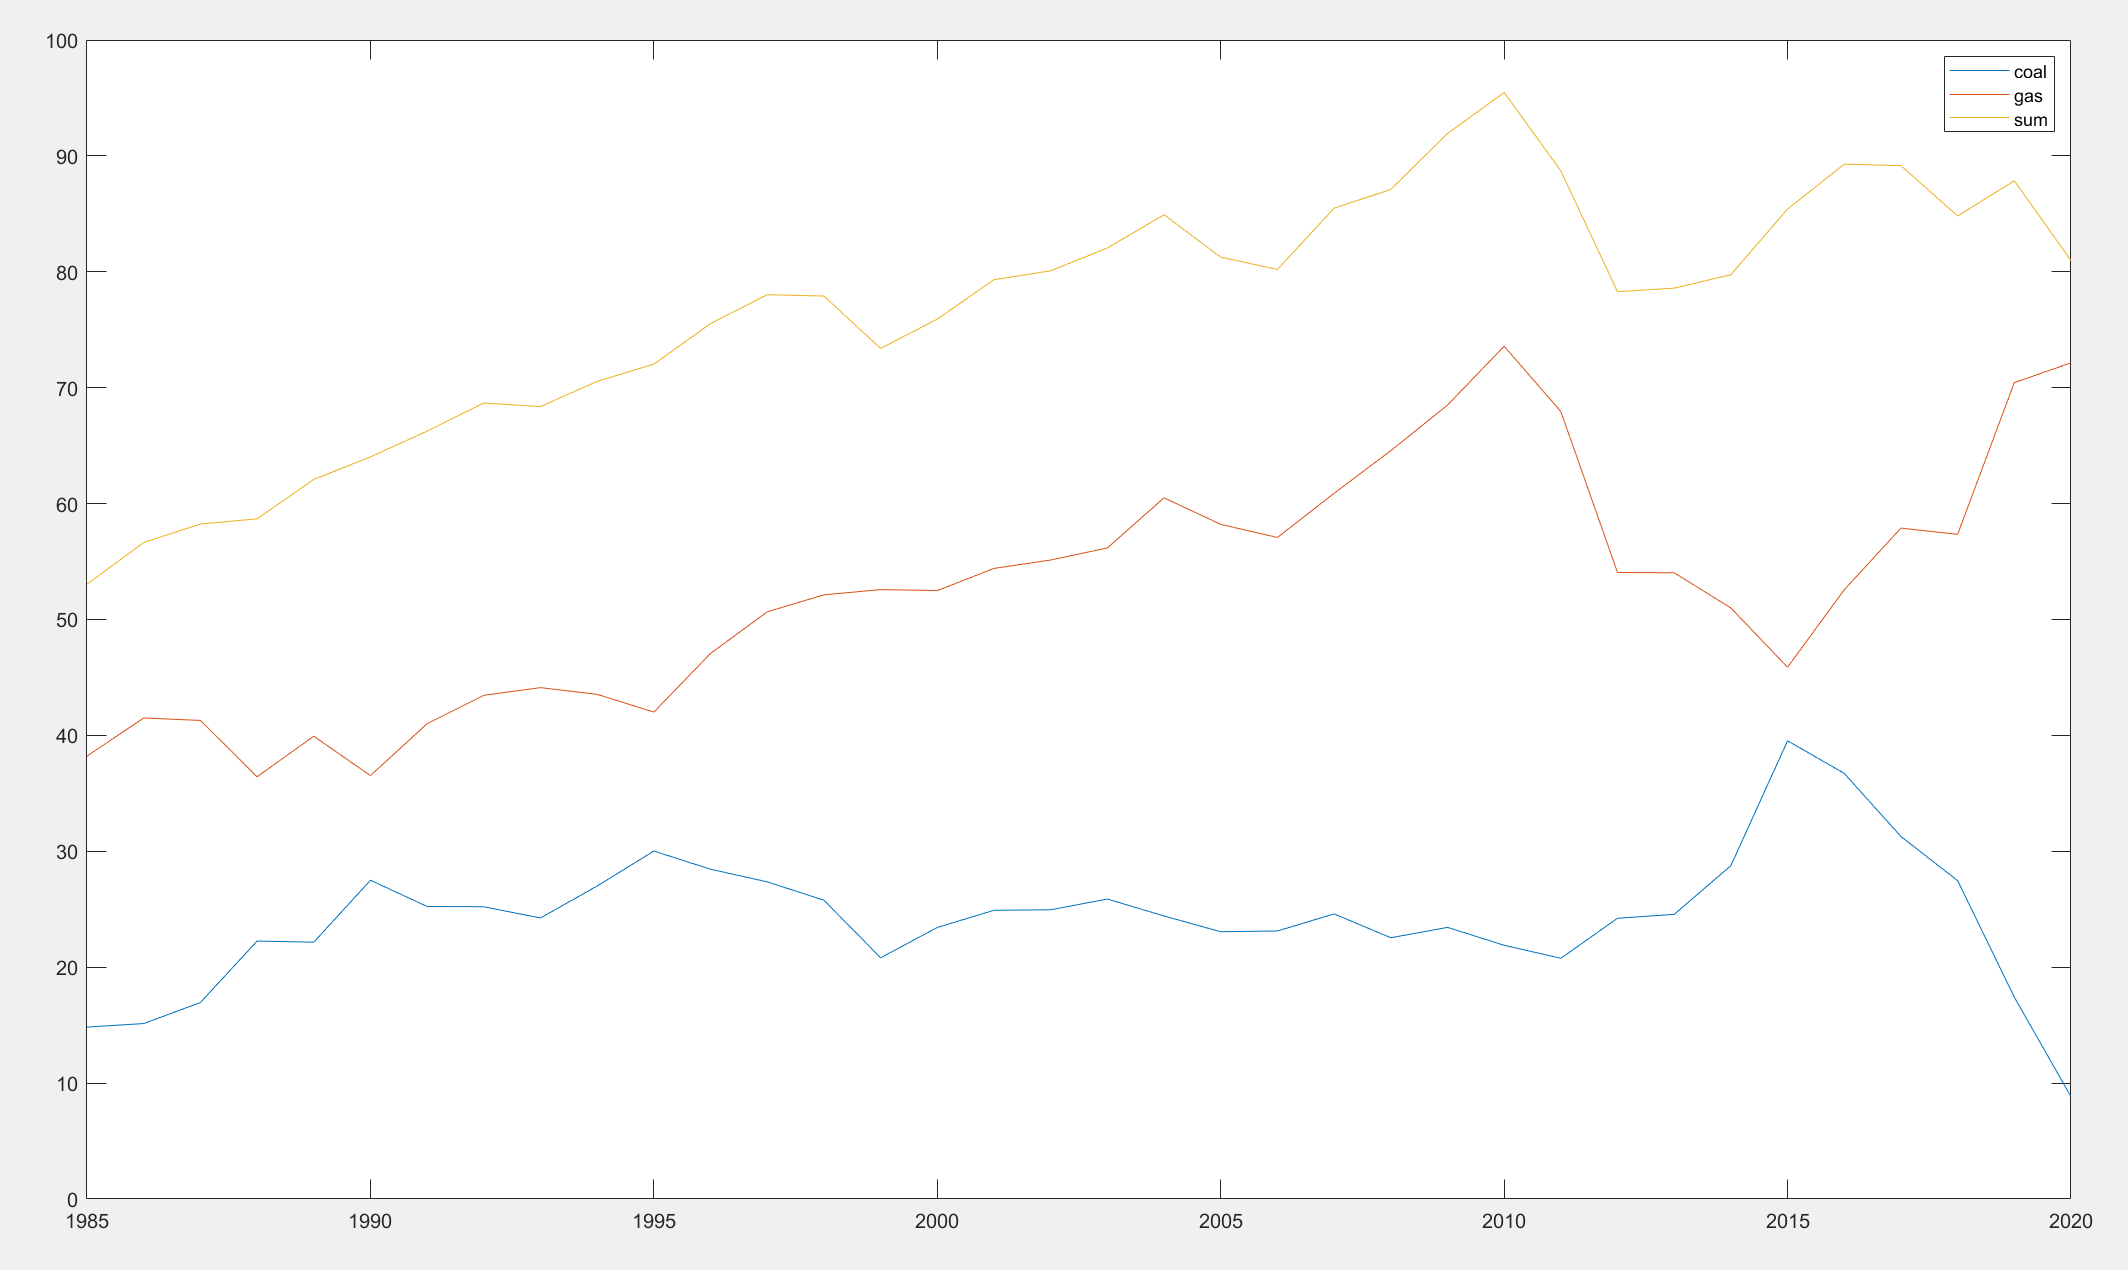
\includegraphics[width=.7\textwidth]{coal oil and gas.png}
	\caption{coal oil and gas}
	\label{fig_2}
\end{figure}

对于荷兰总发电量的预测模型,我们做了如下分析。从相关文献中可以得到,灰色系统理论是研究解决灰色系统分析、建模、预测、决策和控制的理论。而灰色预测模型作为一种预测方法,是对灰色系统所作的预测。相比于灰色预测模型GM(1,1),目前常用的其他预测模型如时间序列预测法在遇到外界发生较大变化,往往会有较大偏差,而通过对数据的分析,其中存在间歇性的较大波动,因此不适用于本案例;微分方程模型需要以局部规律的独立性假定来建立模型,但局部规律具有不确定性和波动性,预测结果差距较大并且微分方程的接比较难得到;差分方程模型预测结果稳定性不高,且预测各组成部分变化规律不一致甚至完全相反;神经网络模型需要大量数据进行机器学习训练才能得到比较准确的值,而用于本次预测的数据量较少,不足以供神经网络模型训练出准确结果。

综合上述分析,对于荷兰总发电量的预测,我们选择使用灰度预测模型GM(1,1)作为小样本预测问题的有效工具。

\begin{itemize}
	\item 模型的建立
\end{itemize}

为了保证本模型的可行性,需要对数据进行预处理。在荷兰发电总量预测过程中,参考数据为1985年至2020年共36年的发电量数据,对这些数据后除操作得到处理后的数组$x(k)$,通过程序计算数列的级比,即$\lambda(k)$在$(0.9375,1.029)$之间,$k=1,2,...35$。这里n=35,显然级比落在$(e^{-\frac{2}{n+1}},e^{-\frac{2}{n+2}})$之间,可以说明数列$x(k)$可以作为灰度预测模型GM(1,1)的数据来预测。

\begin{itemize}
	\item 模型的求解
\end{itemize}

首先进行筛选后数据的预处理,为了减小数据的起伏波动,将数据累加
\\由原始数据序列$x^{(0)}$计算一次累加序列$x^{(1)}$;\\
其中
\[
	x^{(i)}(i)=\sum_{j=1}^ix^{(0)}(j)\qquad(i=1,2,\cdots ,N)
\]
\\
按照GM(1,1)灰度预测模型,对$x(k)$数组进行累加求和,得到\[x(1)=(62.9750,130.14,198.59,...3398.0)\]

构造数据矩阵$B$及数据向量$Y$

\qquad$B=\begin{bmatrix}-\frac{1}{2}(x^{(1)}(1)+x^{(1)}(2)) & 1\\-\frac{1}{2}(x^{(1)}(2)+x^{(1)}(3)) & 1\\ \vdots & \vdots \\-\frac{1}{2}(x^{(1)}(35)+x^{(1)}(36)) & 1\end{bmatrix}$, \qquad $Y=\begin{bmatrix}x^{(0)}(2)\\x^{(0)}(3)\\ \vdots \\x^{(0)}(36) \end{bmatrix}$

我们经过分析,认为可以假设$x^{(1)}$满足微分方程

\begin{equation} 
  \frac{dx^{(1)}}{dt}+ax^{(1)}=u\label{math_1} 
\end{equation}\\
这其中的$u$称为内生控制灰数;$a$为发展灰数\\解初值方程
建立矩阵$\mathbf{B , y}$;\\
求逆矩阵$ \mathbf{B}^T\mathbf{B}^{-1} $;\\
根据
\begin{equation} 
	\hat{\mathbf{U}} = \begin{bmatrix}\hat{a}\\ \hat{u}\end{bmatrix}=(\mathbf{B}^T\mathbf{B})^{-1}\mathbf{B}^{T}y \label{math_2} 
\end{equation}
求得估值$\hat{a}=-0.0162$和$\hat{u}=69.7205$\\
根据时间响应方程
\begin{equation}
	\hat{x}^{(1)}(k+1)=(x^{(1)}(1)-\frac{\hat{u}}{\hat{a}})e^{-\hat{a}k}+\frac{\hat{u}}{\hat{a}}
\end{equation}
取$\hat{x}^{(1)}(1)=\hat{x}^{(0)}(1)=x^{(1)}(1)=62.9750$\\
计算拟合值$\hat{x}^{(1)}(i)$,\\ 然后再减还原运算\\
\begin{equation} 
\hat{x}^{(0)}(i)=\hat{x}^{(1)}(i)-\hat{x}^{(1)}(i-1)  \qquad  (i=1,2,\cdots ,N) \bm ; \label{math_3}  
\end{equation}
得到$\hat{x}^{(0)}=(\hat{x}^{(0)}(1),\hat{x}^{(0)}(2),\cdots ,\hat{x}^{(0)}(36))=(62.9750,71.3159,\cdots,123.6711)$

根据级比$\lambda(k)\in[0.9375,1.029]$和发展系数a求出相应的级比偏差\[\rho(k)=1-(\frac{1-0.5a}{1+0.5a})\lambda (k) \in [-0.0054,0]\]

所得到的结果远远小于$\rho(k)<0.1$的标准,此模型达到极高的精度要求。进一步分析发现在2007年至2011年的真实值高于预测值,2012年至2015年真实值低于预测值,但最后预测结果按照精度检验等级表,后验差比值C为0.28729,系统预测精度为最高精度。\upcite{xiaoai}

综上可知,本次灰度预测模型GM(1,1)以较高精度实现预测,借助MATLAB软件预测未来的总发电量,对荷兰总发电量预测结果如\textbf{表\ref{table_1}},MATLAB软件对荷兰总发电量预测的折线图如\textbf{图\ref{fig_3}}。


	\begin{table}[]
		\centering
		\begin{tabular}{|c|c|c|c|c|c|c|}
		\hline
		\textbf{年份} & \textbf{2021} & \textbf{2022} & \textbf{2023} & \textbf{2024} & \textbf{2025} & \textbf{2026} \\ \hline
		发电量($TWh$) & 125.68        & 127.74        & 129.82        & 131.94        & 134.09        & 136.28        \\ \hline
		\textbf{年份} &\textbf{2027} & \textbf{2028} & \textbf{2029} & \textbf{2030} & \textbf{2031} & \textbf{2032} \\ \hline
		发电量($TWh$) &138.51        & 140.77        & 143.07        & 145.4         & 147.78        & 150.19        \\ \hline
		\textbf{年份} &\textbf{2033} & \textbf{2034} & \textbf{2035} & \textbf{2036} & \textbf{2037} & \textbf{2038} \\ \hline
		发电量($TWh$) &152.64        & 155.13        & 157.66        & 160.24        & 162.85        & 165.51        \\ \hline
		\textbf{年份} &\textbf{2039} & \textbf{2040} & \textbf{2041} & \textbf{2042} & \textbf{2043} & \textbf{2044} \\ \hline
		发电量($TWh$) &168.21        & 170.96        & 173.75        & 176.59        & 179.47        & 182.4         \\ \hline
		\textbf{年份} &\textbf{2045} & \textbf{2046} & \textbf{2047} & \textbf{2048} & \textbf{2049} & \textbf{2050} \\ \hline
		发电量($TWh$) &185.38        & 188.4         & 191.48        & 194.6         & 197.78        & 201.01        \\ \hline
		\end{tabular}
		\caption{荷兰总发电量预测结果}
	\label{table_1}
		\end{table}

		\begin{figure}[!h]
			\centering
			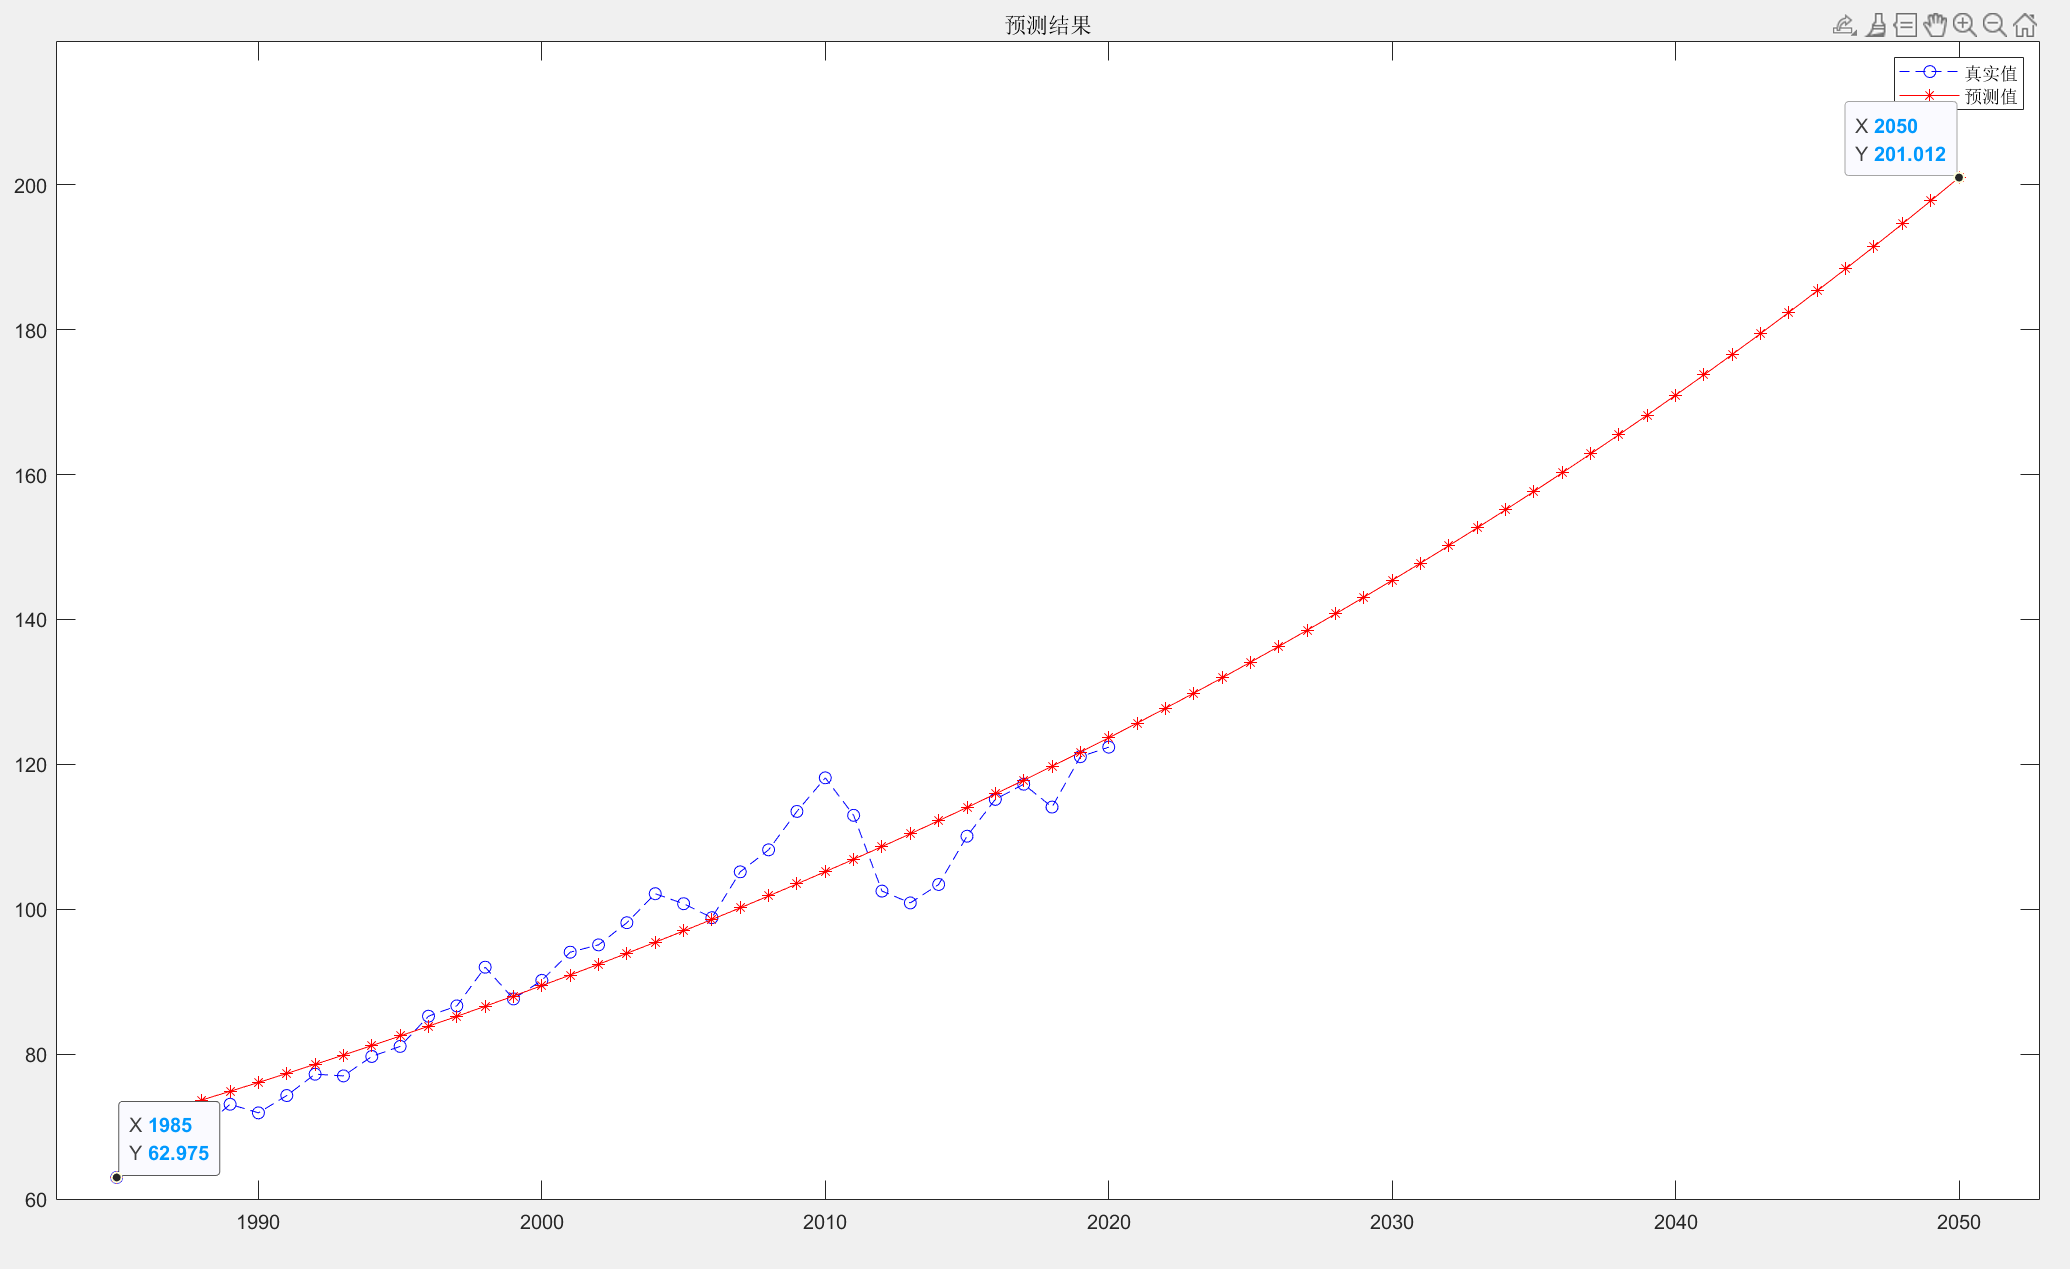
\includegraphics[width=.7\textwidth]{发电量预测.png}
			\caption{荷兰发电量预测}
			\label{fig_3}
		\end{figure}

\begin{itemize}
	\item \textbf{碳排放量预测}
\end{itemize}

\begin{itemize}
	\item 模型的准备
\end{itemize}
荷兰年碳排放量的数据是从\href{http://www.bp.com/statisticalreview}{BP energy partners}中得到的,通过对荷兰年碳排放的变化情况可以看出,荷兰年碳排放量并不平稳变化,中间存在数据的突变,例如在1993年,1996年,2005年和2016年都有碳排放的数据高峰,其中2005年碳排放达到历史最高水平。由于政策的影响,未来荷兰的碳排放减少速率会有所提升,但随着科技的完善,限制了进一步减少碳排放。由于1985年至2020年中出现多次科技突破、历史变革,1985至2010年的数据仅作保留参考,不参与实际的模型构建。通过对荷兰碳排放各组分分析,发现煤、原油、天然气这类传统能源提供了近100\%的碳排放量,而其他能源碳排放量远远低于传统能源,因此,在将模型构建的过程中,我们近似的假设荷兰碳排放量完全来源于传统能源。而进一步对传统能源碳排放量进行分析,发现虽然各年碳排放量变化较大,但主要变化影响因素来源于天然气,煤和原油碳排放量较稳定,而天然气受国际市场价格、供给等因素影响,在此对政治影响不做考虑。

\begin{itemize}
	\item 模型的建立
\end{itemize}
对于荷兰碳排放量的预测,适合有GM(1,1)灰度预测模型,时间序列非平稳型预测模型和神经网络预测模型。本次建模对三个预测模型做了不同程度的尝试,最后的结果和精度检验都表示出,以GM(1,1)灰度预测模型为基础的对碳排放来源加权平均最小二乘拟合法表现出较好的精度。

在使用BP神经网络模型进行预测时,需要将数据分为训练集和测试集两部分,训练集用于机器学习,通过大量数据迭代训练,使机器具备学习预测的能力,通过改变自变量得到想要的预测结果。但是结果表明,BP神经网络学习对训练集预测较为准确,但对测试集误差较大,经过反复学习仍未达到理想的效果,我们认为是所给的训练集数据过少,无法满足BP神经学习所需要的数据量。而时间序列非平稳型预测模型虽然适合按时间周期性变化的数据,但碳排放量数据存在时间对碳排
放量影响大小不一致的情况,受外界干扰显著。结果可想而知并不理想。(如图片\ref{fig_{4}},图片\ref{fig_{5}})

		\begin{figure}[!h]
			\centering
			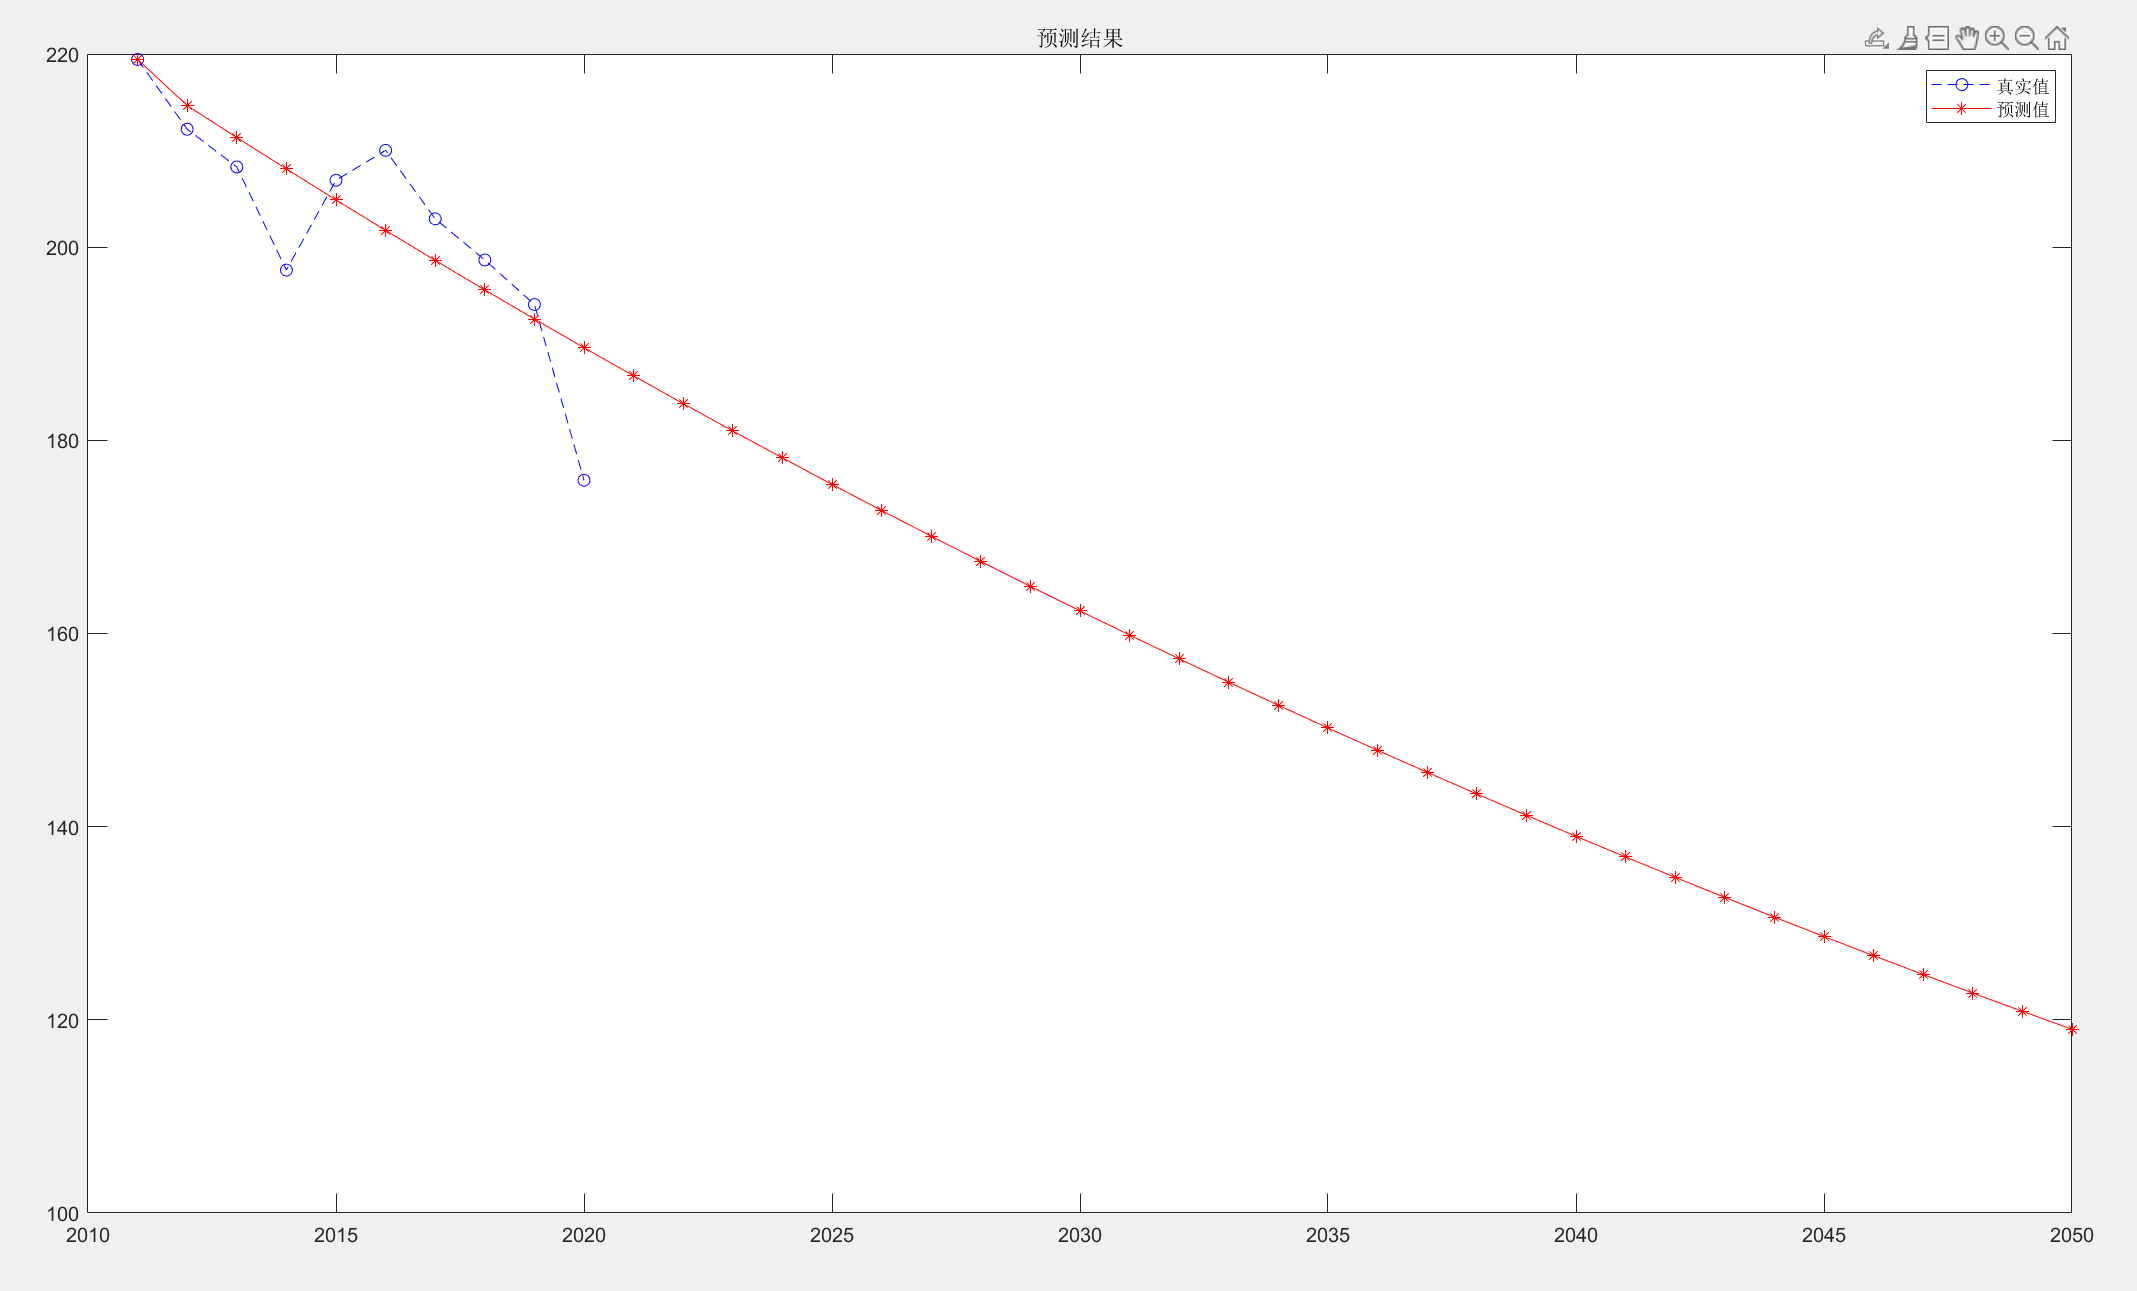
\includegraphics[width=.7\textwidth]{02碳排放预测修改前.png}
			\caption{碳排放预测修改前}
			\label{fig_{4}}
		\end{figure}
		\begin{figure}[!h]
			\centering
			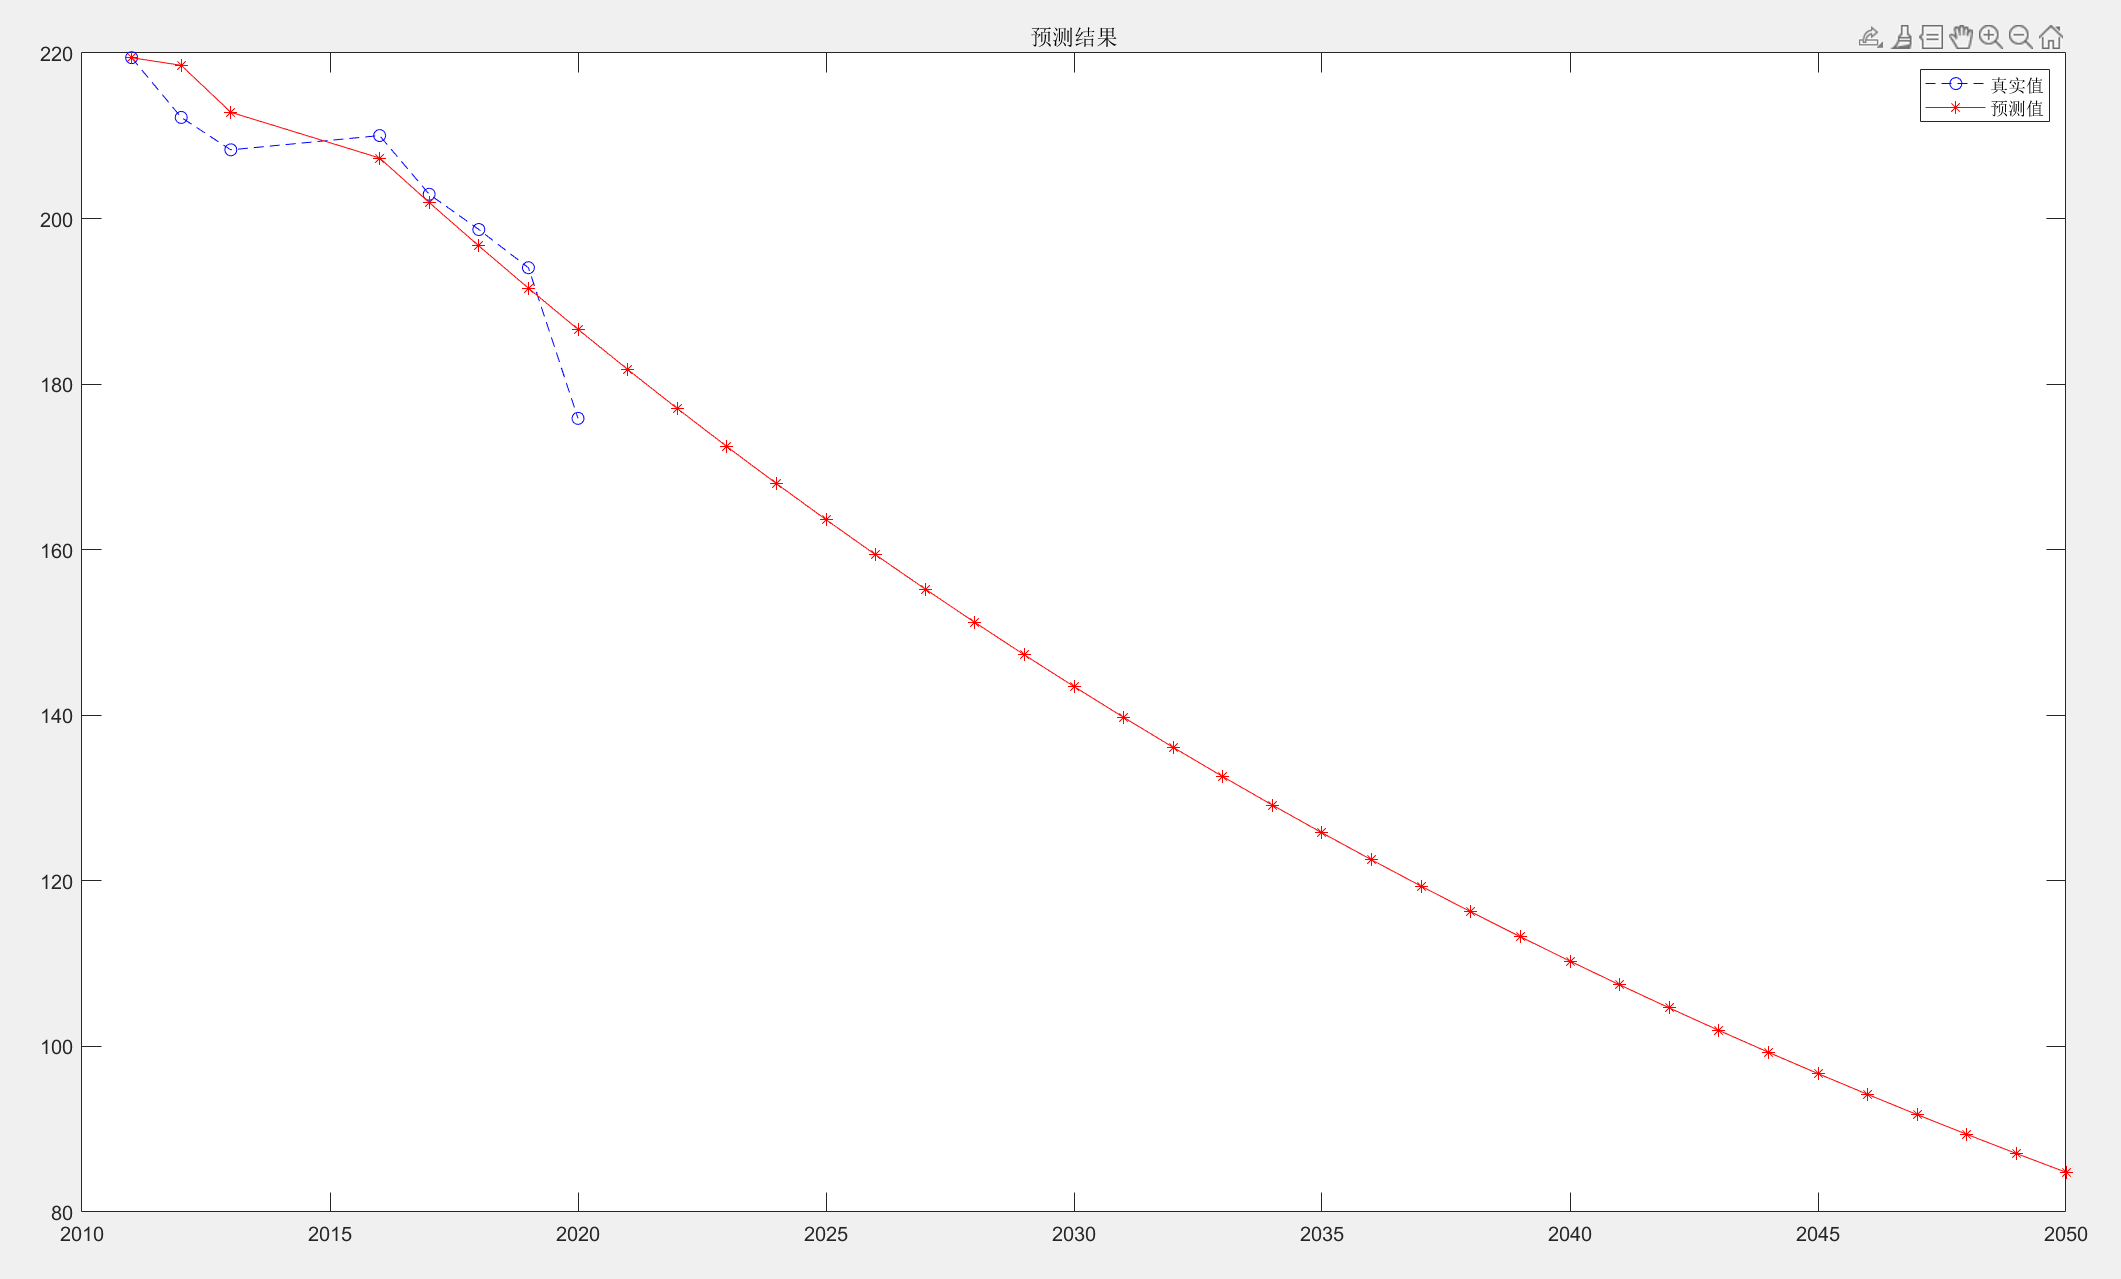
\includegraphics[width=.7\textwidth]{02碳排放预测修改后.png}
			\caption{碳排放预测修改后}
			\label{fig_{5}}
		\end{figure}

我们对碳排放的数据进行了筛选,过于偏离拟合得到的曲线的数据我们对其进行了分析。发现其(2014-2015)的
偏离是因为外部经济因素影响导致的能源结构临时波动调整。该次能源结构冲击涉及到了整个欧洲。从当时的新闻报道可以看出
“2013年欧洲多个天然气发电站因严重亏损倒闭”,“受煤炭价格下降影响,2014年荷兰能源企业煤炭使用量同比增长5\%。荷兰29\%的电力消耗来自于化石能源,而煤炭产生的二氧化碳是天然气的两倍。”
我们综合分析,根据【模型假设\ref{jiashe}】“认为该国家会全力执行现有的碳中和战略”,预测模型中的国家不会受到过多经济因素的影响。因此为了模型预测的精确性我们剔除了2014-2015年的碳排放数据。

因此在多次试错之后,仍然回归到GM(1,1)灰度预测模型中,但本次直接使用灰度预测模型也并没有得到理想的结果,经过对数据的分析,我们有以下几点看法:
\begin{enumerate}
	\item 数据前20年的变化起伏过大,对于适合小样本,中短期预测的灰度预测模型来说难以得到适合后20年的预测,导致预测方差过大,精度不高。
	\item 在后20年的数据中,主要碳排放来源的各类传统能源碳排量变化较大,如果不细分考虑,最后的结果很难准确合理。
	\end{enumerate}

综上,我们在进行模型构建时做出\textbf{创新改进},考虑更接近2020年的数据,并对各组分分别考虑处理。

\begin{itemize}
	\item 模型的求解
\end{itemize}

在GM(1,1)灰度预测基础上,分别模拟出煤、原油、天然气的预测值(如图\ref{fig_{10}}。再对三个量作权重分配,权重分配依据为三种能源在发电量中的占比,因为三种能源在发电量到使用量存在一个比例系数,从使用量到碳排放存在另一个比例系数,所以可以通过线形变化将三种能源发电量与碳排放量相关联,即$e(x)=kg(x)$,x代表三种能源。通过灰度预测GM函数求出三种能源发电量预测结果之和$t=emm1+emm2+emm3$,其中$emm1=GM(num1)$,$emm2=GM(num2)$,$emm3=GM(num3)$。得到转化因子$p(i)=\frac{t(i)}{t(i)}$;再将转化因子与通过GM灰度预测模型进行结果的预测拟合,提高精度。最后将转化因子与原始数据结合得到预测总碳排放量如表\ref{table_{2}}和图\ref{fig_{3}}
\begin{figure}[!h]
	\centering
	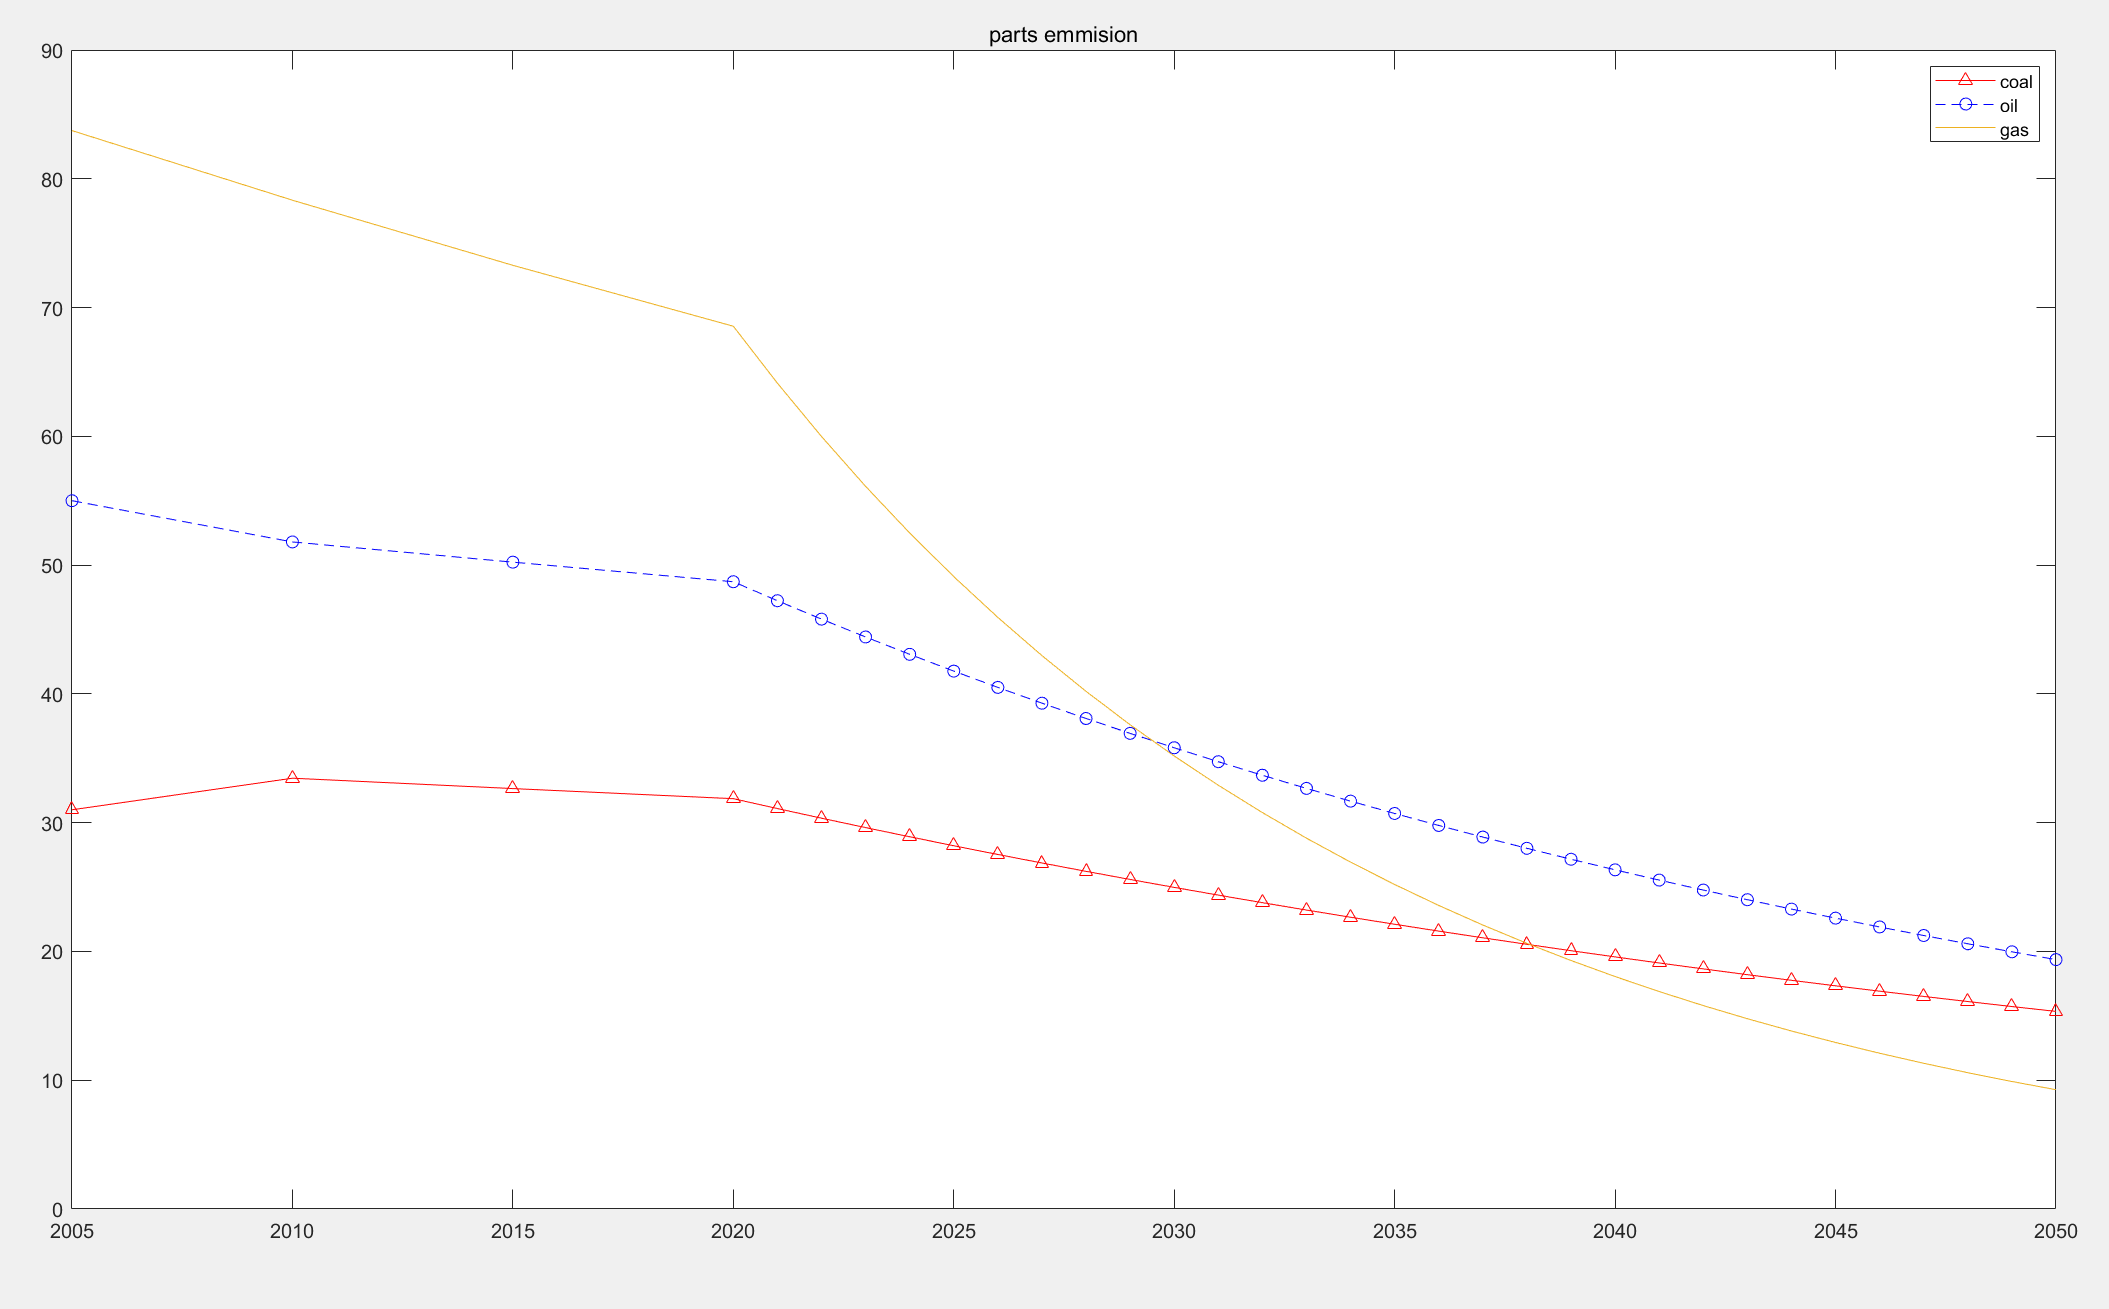
\includegraphics[width=.7\textwidth]{煤炭石油天然气碳排放预测.png}
	\caption{煤炭石油天然气碳排放预测}
	\label{fig_{10}}
\end{figure}
\begin{table}[]
	\centering
	\begin{tabular}{|c|c|c|c|c|c|c|}
	\hline
	\textbf{年份} &\textbf{2021} & \textbf{2022} & \textbf{2023} & \textbf{2024} & \textbf{2025} & \textbf{2026} \\ \hline
	碳排放($Mt$)&152.98        & 148.8         & 144.76        & 140.84        & 137.05        & 133.38        \\ \hline
	\textbf{年份} &\textbf{2027} & \textbf{2028} & \textbf{2029} & \textbf{2030} & \textbf{2031} & \textbf{2032} \\ \hline
	碳排放($Mt$)&129.83        & 126.39        & 123.06        & 119.83        & 116.71        & 113.68        \\ \hline
	\textbf{年份} &\textbf{2033} & \textbf{2034} & \textbf{2035} & \textbf{2036} & \textbf{2037} & \textbf{2038} \\ \hline
	碳排放($Mt$)&110.75        & 107.92        & 105.17        & 102.51        & 99.94         & 97.45         \\ \hline
	\textbf{年份} &\textbf{2039} & \textbf{2040} & \textbf{2041} & \textbf{2042} & \textbf{2043} & \textbf{2044} \\ \hline
	碳排放($Mt$)&95.03         & 92.69         & 90.43         & 88.23         & 86.1          & 84.05         \\ \hline
	\textbf{年份} &\textbf{2045} & \textbf{2046} & \textbf{2047} & \textbf{2048} & \textbf{2049} & \textbf{2050} \\ \hline
	碳排放($Mt$)&82.05         & 80.12         & 78.25         & 76.43         & 74.68         & 72.98         \\ \hline
	\end{tabular}
	\caption{荷兰总碳排放量预测结果}
	\label{table_{2}}
	\end{table}
	\begin{figure}[!h]
		\centering
		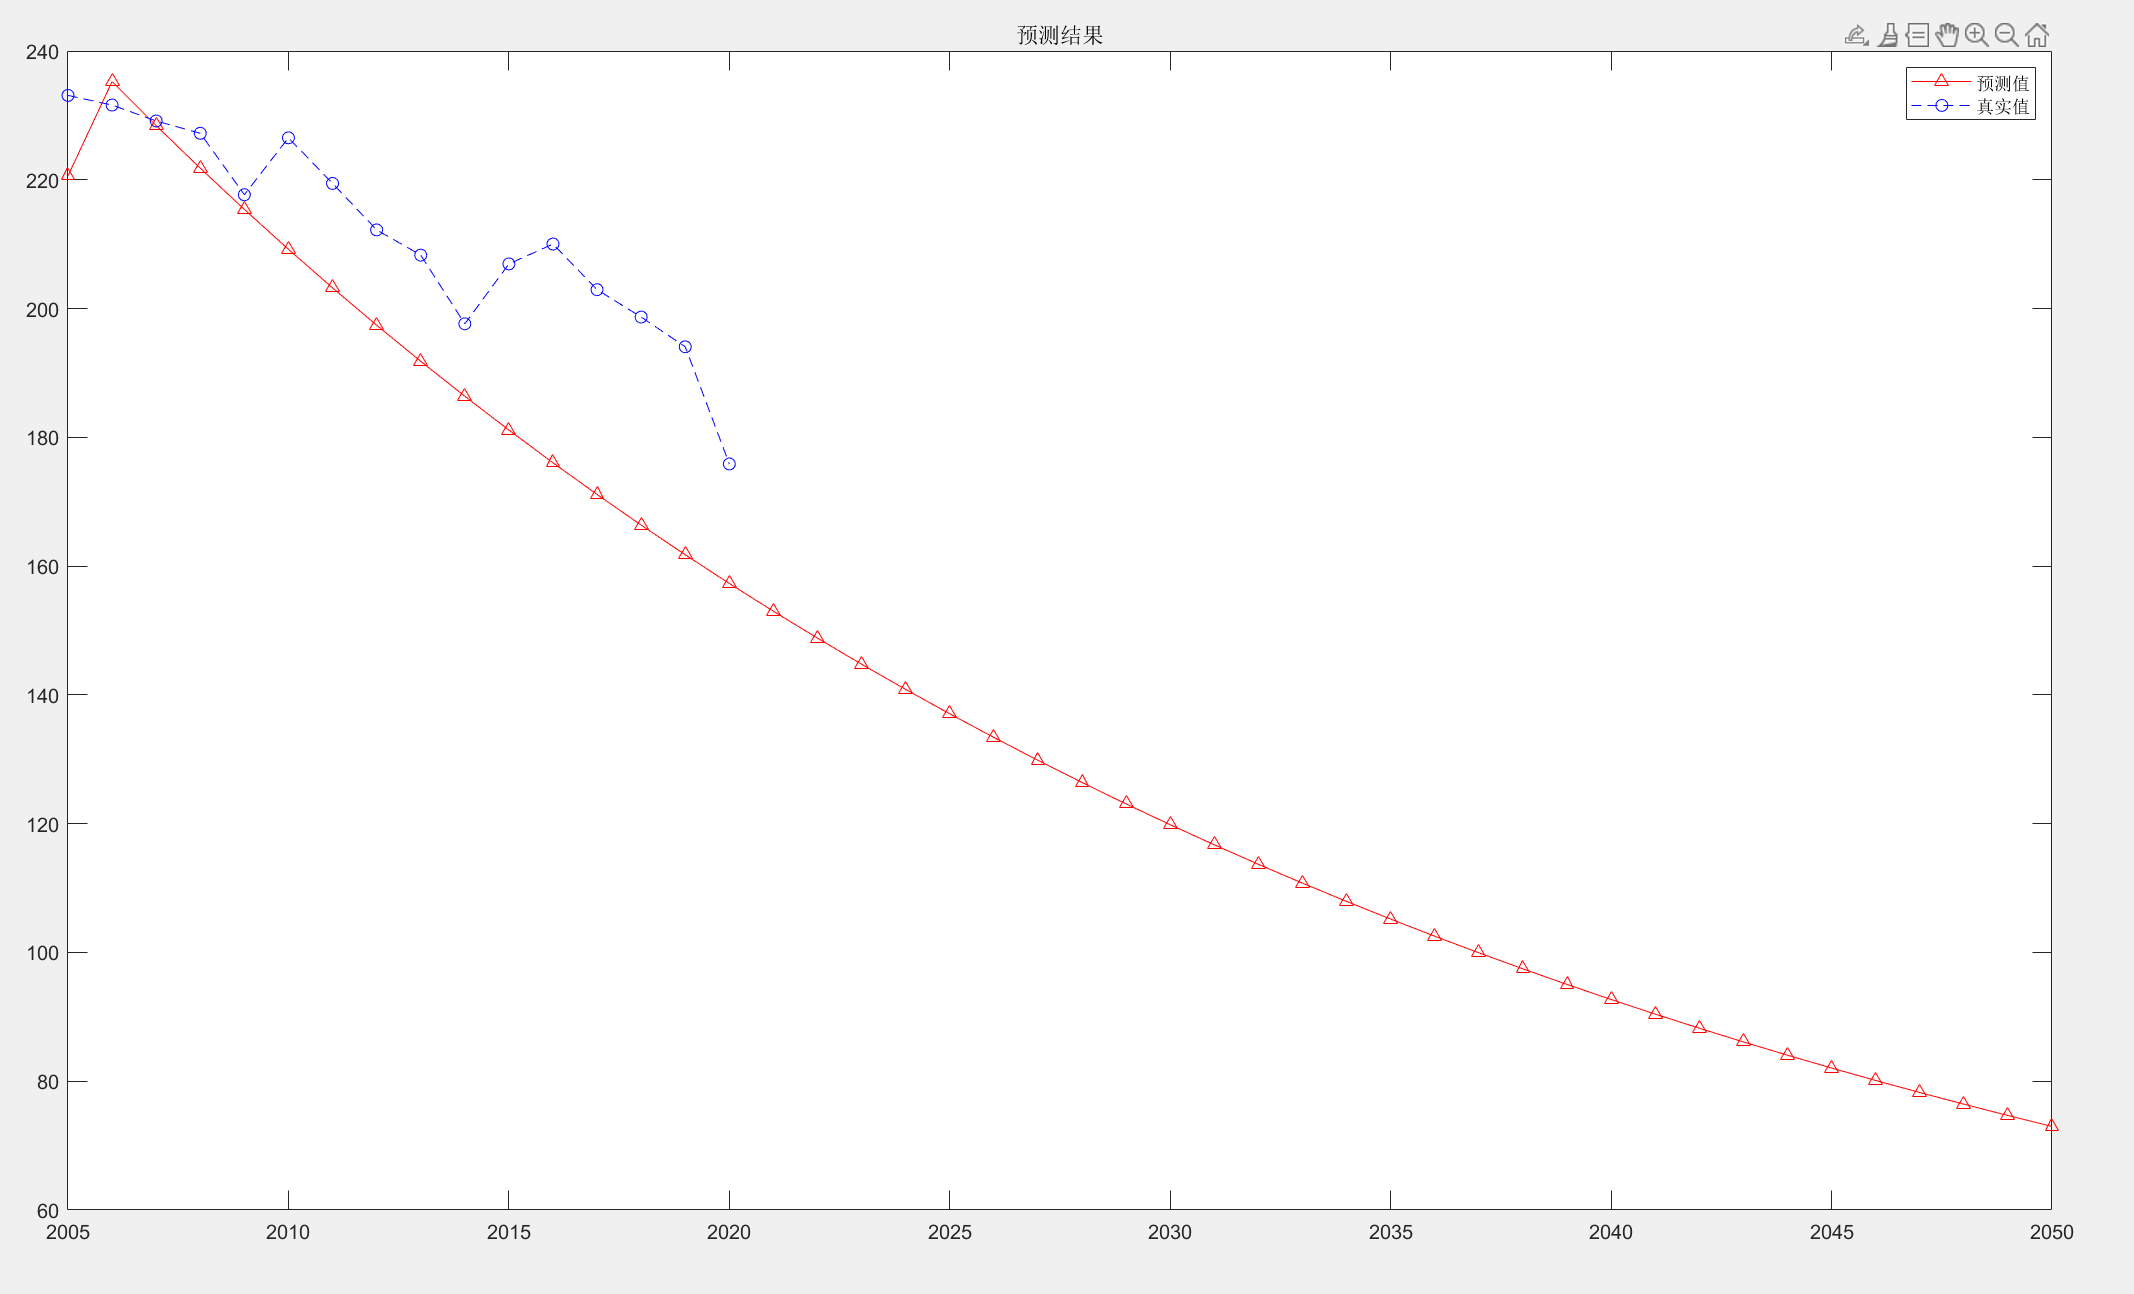
\includegraphics[width=.7\textwidth]{03carbon emmision.png}
		\caption{carbon emmision}
		\label{fig_{3}}
	\end{figure}

\subsection{分析荷兰为了要在2050年实现零排放该如何建设碳吸收能力}
\subsubsection{问题分析}
问题二要求我们广泛浏览官方文件并收集相关数据报道,根据荷兰的国家地理环境特征和技术发展情况,分析选取可行的碳吸收手段
并加权计算对应碳吸收量。我们下面列举的碳吸收举措是建立在检索到的荷兰政府项目和论文基础上的延展和具体化。
\subsubsection{模型建立与求解}
\begin{itemize}
	\item \textbf{CCS和CCUS建设}
\end{itemize}
\begin{figure}[!h]
	\centering
	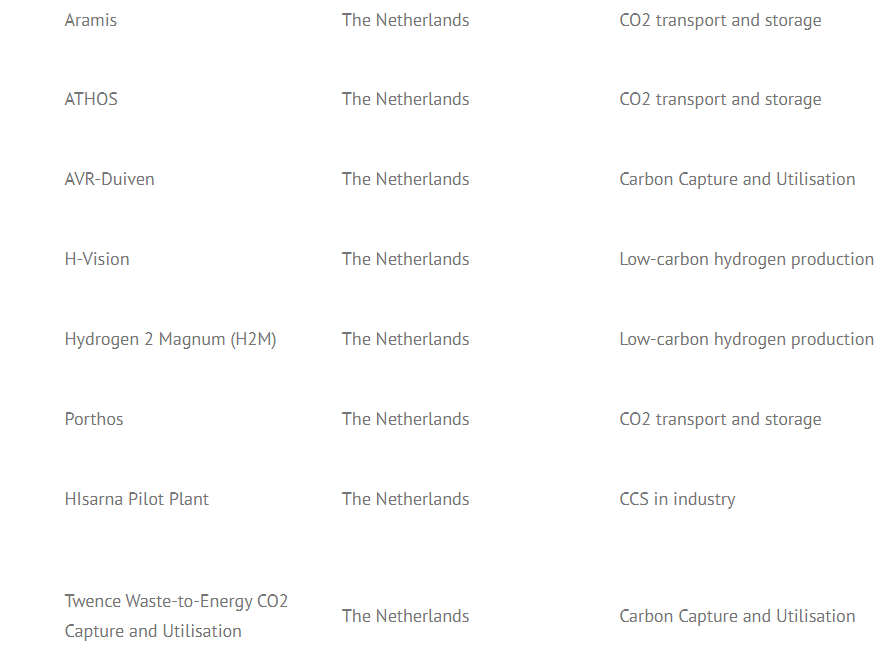
\includegraphics[width=.7\textwidth]{CCS.png}
	\caption{CCS and CCUS projects in Nederland}
	\label{fig_9}
\end{figure}

目前荷兰国内有许多在建的二氧化碳吸收、利用和储存(CCS/CCUS)项目,(如图 \ref{fig_9} )根据气候协议,内阁已经同意,到2030年工业排放减排量的一半将通过CCS实现。CCS和CCUS是目前减少空气中二氧化碳含量最直接迅速的方式,因短时间内难以实现能源减排和固碳技术的突破性进展,CCS和CCUS项目在本文的预测年限内很可能会保持为一个主要的碳吸收途径。

以荷兰国内目前最大的在建项目Porthos为例,政府将在海上建设约20千米运输管道,用于从荷兰鹿特丹港口运输二氧化碳至北海海底的储存库。Porthos项目建成后,将可以每年储存二氧化碳约250万吨,累计15年,总计封存3700万吨二氧化碳,项目计划在2024-2025年投入使用。除封存外,二氧化碳也将被应用于其他领域,包括使用$CO_2$种植花卉,蔬菜和植物等作物,应用于油气开采等等。如AVR-Duiven项目致力于捕获处理工业残余废物过程中产生的二氧化碳用于农业和花卉养殖,在可预见的未来将实现年捕获超过200万吨的二氧化碳。

因为目前CCS和CCUS项目大多处于在建和试运营阶段,其碳吸收数据均为官方网站上的预估值,实际数据量过少,故该部分没有采用数学建模分析。我们统计了上述项目给出的年吸收量,估计其最终效果为每年可吸收二氧化碳约1000-1200万吨,随着技术的成熟和项目的扩建,我们乐观估计,到2050年,CCS和CCUS项目提供的年吸收水平将达到2500万吨。(如图\ref{fig_10})

\begin{figure}[!h]
	\centering
	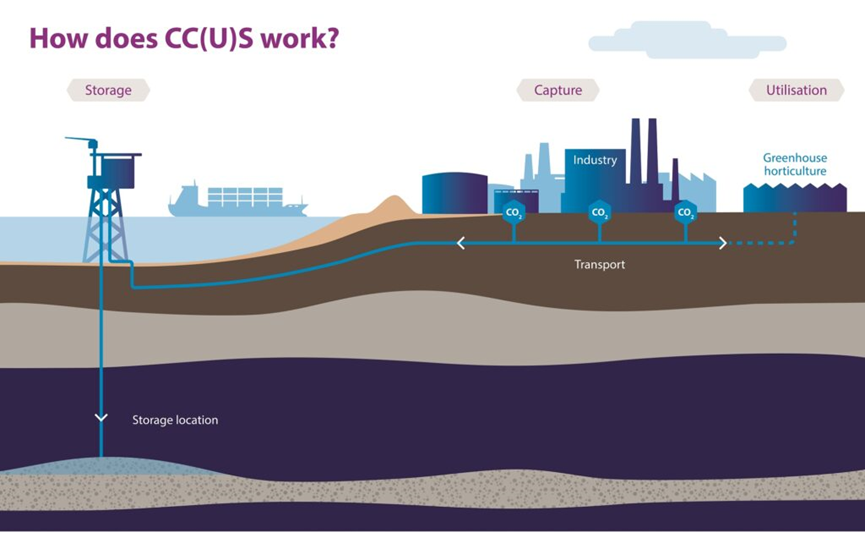
\includegraphics[width=.7\textwidth]{CCS2.png}
	\caption{the operation mode of CC(U)S}
	\label{fig_10}
\end{figure}


\begin{itemize}
	\item \textbf{森林和草地碳汇}
\end{itemize}

荷兰国土面积41864平方公里,属温带海洋性气候,冬季温和,一月平均温在0℃左右;夏季平均气温约15—20℃.年降雨量700—775mm,不同季节雨量稍有波动,但没有极端的干旱季节,以西北大西洋植物区系为主。人工植被是荷兰的主要植被类型,复盖面积最大,包括占全国面积71\%的人工草地和农业植被,还有园林绿化与庭园,森林主要分布在东、南部,以栎桦林、山毛榉栎林、桤木林为主,乔木层主要树种还有欧洲松、欧山毛榉、桦木、榛子,灌木层有花楸、乌饭树、山楂等,草木层以蕨占优势。\upcite{2-1}

我们收集了荷兰最近几年的森率覆盖率,采用数学建模拟合数据,得到2050年荷兰国家森林覆盖率的预估值为11.85\%,即到2050年,荷兰的森林面积将达到4960.88平方公里,合496088公顷。我们假设树木的年龄和生长状态是符合正态分布规律的,综合计算下得到每公顷的森林可以储存约10吨二氧化碳。这意味着,到2050年,全国的森林可以吸收约5 Mt二氧化碳。
\begin{figure}[!h]
	\centering
	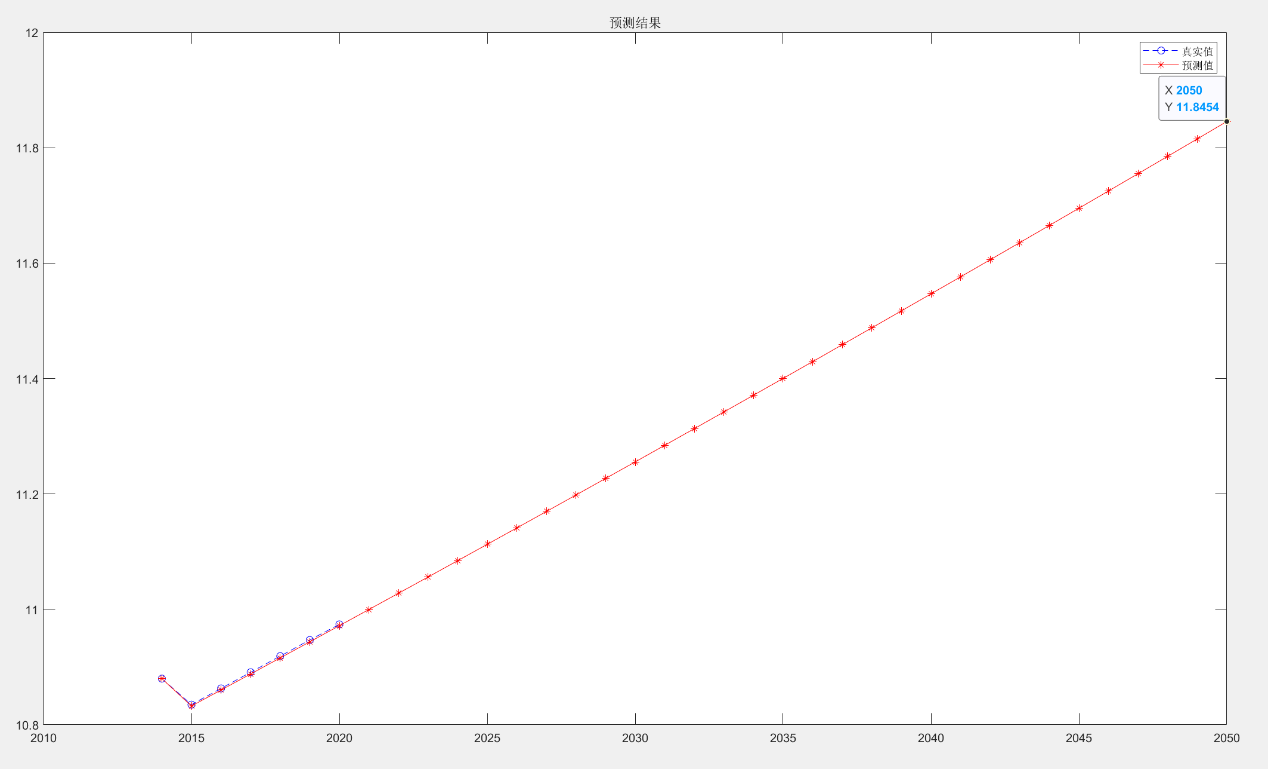
\includegraphics[width=.7\textwidth]{for.png}
	\caption{forest coverage rate}
	\label{for}
\end{figure}

此外,荷兰拥有约276000公顷的湿地,这些湿地也是有效的碳吸收生态系统。通过提高水位,每年每公顷湿地将减少5至15吨的二氧化碳排放。到2050年,草地碳汇可以提供3Mt的碳吸收值。

\begin{itemize}
	\item \textbf{海洋碳汇}
\end{itemize}

根据联合国《蓝碳》报告,地球上55\%的生物碳捕获是由海洋生物完成的,这些海洋生物包括浮游生物、细菌、海藻、盐沼植物和红树林,主要集中在沿海生态系统。海洋负排放潜力巨大,是当前缓解气候变暖最具双赢性、最符合成本-效益原则的途径。荷兰有很长的海岸线,临海水域面积约154011平方公里,海洋碳汇资源丰富,作为发达国家,具有建设和应用海洋碳汇完成本国减排目标的能力。但是考虑到荷兰历史上多次填海造陆,海滨湿地数量锐减,沿海污染严重,且大量开发海上风电站,干扰海洋生态,虽然1990年政府出台《自然政策计划》决定恢复沿海水域生态,但是滨海生态综合恢复速度慢。综上,我们认为荷兰海域在未来30年内的碳吸收能力要低于世界平均水平,且并非所有海洋提供的碳吸收可以直接反映于国内二氧化碳当值,保守预估,我们取荷兰海域的30\%用于进行国内碳吸收建设,最终吸收效率取世界平均水平的40\%。\upcite{2-2}

根据卫星遥感归一化差异植被指数(Normalized Difference Vegetation Index )的估算结果,海洋的年平均初级生产力为140 $g$\quad$C·m^{-2}·a^{-1}$,年初级生产量为48.5 Gt C/a。\upcite{2-3}世界沿海水域只占全球海洋总面积的7\%,即25.2百万平方千米,我们所取的有效水域面积为世界总面积的0.18\%,每年所得碳吸收值约为35Mt。

综合上述,采用CCS/CCUS项目、森林碳汇和海洋碳汇作为碳吸收的主要手段,可以提供大致68Mt的二氧化碳吸收值,加上其他未提及的一些手段,大致可以满足抵消50年的碳排放量。
\subsection{判断荷兰2050年实现零排放的目标是否切实可行}
\subsubsection{问题分析}
在上述4.1和4.2两问中,我们已经得到了2050年的二氧化碳排放预计水平和基于技术发展预期的可以与碳排放相抵的碳吸收建设方案,故在本问中,我们将着重分析这一方案在经济领域的成本,与荷兰的国民生产总值(GDP)比较,以此作为荷兰2050年实现零排放目标的可行性判断依据。
\subsubsection{模型建立与求解}
\begin{itemize}
	\item \textbf{CC(U)S项目成本核算}
\end{itemize}

经济性始终是CCS可行性的主要影响因素。目前荷兰主要采用的碳捕集手段是将二氧化碳注入油气层或煤气层封存,虽然目前的项目多为直接使用现成的油气田,但是从发展的眼光看,仍旧存在储存设备研发及建设的开发成本以及管道和平台的铺设成本,预估为20亿美元。

此外CCS的主要成本还包括捕获与压缩、运送、封存、检测四部分。\upcite{3-1}全球商业化运营的CCS项目成本约为60-90美元/吨碳。其中陆地地质封存成本约为0.5~5美元/吨碳,海洋地质封存的成本约为6~12美元/吨碳,管道输送的成本约1~8美元/吨碳,监测成本0.05~0.1美元/吨碳, $CO_2$捕获与压缩的成本约为30~60 美元/吨碳。\upcite{3-2}由上述4.2.2,我们估测的年二氧化碳吸收量为2500万吨,即每年CCS和CCUS项目的二氧化碳处理成本约为22.50亿。

就荷兰工厂碳捕获方面而言,$CO_2$的捕获需要增加额外的能源以保证其实施, 目前工厂利用最成熟的技术可捕获总处理量85\%~95\%的$CO_2$, 与未采用CCS的类似电厂相比, 需要多支出10\%~40\%的能源; 其净结果是,一个采用CCS的电厂相比普通电厂大约能够减少80\%~90\%的$CO_2$排放。能源使用量的增加也将导致环境排放增加, 如固体废弃物。但相对于其他减排措施的利用水平和研究现状, 企业增加CCS系统是经济合算的。

综上,碳捕集项目的合计成本约为 43亿美元。

\begin{itemize}
	\item \textbf{森林碳汇成本核算}
\end{itemize}

由森林覆盖率预测图可知,于2050年森林覆盖率将达到11.85\%,且覆盖率与时间呈线性关系,由此推算出每年森林覆盖率的增长速率为0.029\%/年,合算成面积为1220公顷。由国际统一标准可知,每公顷约种植1000棵树,每棵树种植成本为50美元,即总成本为6100万美元。此外,还有人工草坪、城市绿化、湿地修复等等其他的开销,总计成本预估为2-3亿。

\begin{itemize}
	\item \textbf{海洋碳汇成本核算}
\end{itemize}

目前世界海洋环境相对严峻,海洋生态受到人类活动的破坏,想要可持续发展海洋碳汇,加强海洋的碳吸收和碳固定能力,政府需要加强生态治理并加强相关投资,此外,为了使得海洋碳汇的碳吸收效果较为明显地反映和作用于荷兰的国内二氧化碳当值,还需要提高技术研发的投入成本。上述各项开支总计约15亿美元。

另外,经过对2005年至2020年荷兰GDP拟合分析,预测2050年荷兰GDP将增长至9837.85亿美元。按照2\%预估2050年荷兰政府用于环境治理及监控的支出,即196.76亿美元。我们认为其中的70\%用于包括污水治理、固体废物处理等其他环境治理,剩余的30\%(59亿)用于温室气体治理。综合考虑上述成本投入,累计约合59-60亿,在可接受的置信区间内,说明4.2中谈及的碳吸收能力建设方案是切实可行的。

综上,我们乐观地认为。荷兰可以在2050年实现零排放。
\section{模型的评价}
\subsection{模型的优点}
灰色预测模型该基础本身的优点有:    
\begin{itemize}
\item 不需要大量样本。
\item 样本不需要有规律性分布。
\item 能解决历史数据少、序列的完整性以及可靠性低的问题。
\item 计算工作量小。
\item 定量分析结果与定性分析结果不会不一致。
\item 可用于短期、中长期预测。
\item 灰色预测准确度高。
\end{itemize}

在创新改进之后,我们的模型又有了能够忽略短期经济等影响的优点
\subsection{模型的缺点}
灰色预测模型该基础本身的缺点有:
\begin{itemize}
	\item 只适合近似于指数增长的预测。
	\end{itemize}

	在创新改进之后,我们的模型对初始数据的干净程度要求较灰色预测模型高。


\newpage
\section{参考文献}
%参考文献
\begin{thebibliography}{1.2}%宽度9
	\setlength{\itemsep}{-2mm}
	\bibitem{bib:one}
	邹才能,et al."世界能源转型内涵、路径及其对碳中和的意义". 石油学报, 42.02(2021):233-247. 
	\bibitem{bib:3}
	张雅欣,罗荟霖,王灿.碳中和行动的国际趋势分析[J].气候变化研究进展,2021,17(01):88-97.
	\bibitem{meaning}
	邓旭,谢俊,滕飞.何谓“碳中和”?[J].气候变化研究进展,2021,17(01):107-113.
	\bibitem{bib:4}
	李红卫.生态文明——人类文明发展的必由之路[J].社会主义研究,2004(06):114-116.
	\bibitem{bib:two}
	韩中庚. 数学建模方法及其应用[M]. 高等教育出版社, 2005.
	\bibitem{a}
	刘海洋. LaTeX入门. 电子工业出版社,2013.
	\bibitem{b}
	夏爱生. 数学建模与MATLAB应用. 北京理工大学出版社,2016.
	\bibitem{2-1}
	钟章成,缪世利.荷兰植被概况[J].西南师范大学学报(自然科学版),1986(03):120-124.DOI:10.13718/j.cnki.xsxb.1986.03.019.
	\bibitem{2-2}
	战玉杰. 渤海重金属污染状况及对典型浮游植物生长影响初步分析[D].中国海洋大学,2005.
	\bibitem{3-1}
	张鸿翔,李小春,魏宁.二氧化碳捕获与封存的主要技术环节与问题分析[J].地球科学进展,2010,25(03):335-340.
	\bibitem{3-2}
	Benson SM , Hoversten M, Gasperikova E et al. Monitoringpro-tocols and life-cycle costs for geologic storage of carbon dioxide[M]//Greenhouse Gas Control Technologies 7, Oxford: Elsevier Science Ltd.2005:1259-1264
	\bibitem{2-3}
	Field C B,Behrenfeld M J,Randerson J T,Falkowski P. Primary production of the biosphere: integrating terrestrial and oceanic components. Science,1998,281( 5374) : 237-240.
	\bibitem{kezaishengnengyuan}
	陈奥,黄琨. 我国可再生能源消费与碳排放强度时间序列分析[J]. 科技和产业,2016,16(2):139-145. DOI:10.3969/j.issn.1671-1807.2016.02.026.
	\bibitem{xiaoai}
	霍立田,詹棠森,柳炳祥. 一种基于GM(1,1)的碳排放量预测模型[J]. 信息与电脑,2017(3):53-54. DOI:10.3969/j.issn.1003-9767.2017.03.022.
\end{thebibliography}

\newpage
%附录
\appendix
\section{程序代码}
见压缩包
%\begin{lstlisting}[language=Matlab] 
%kk=2;[mdd,ndd]=size(dd);
%while ~isempty(V)
%[tmpd,j]=min(W(i,V));tmpj=V(j);
%for k=2:ndd
%[tmp1,jj]=min(dd(1,k)+W(dd(2,k),V));
%tmp2=V(jj);tt(k-1,:)=[tmp1,tmp2,jj];
%end
%tmp=[tmpd,tmpj,j;tt];[tmp3,tmp4]=min(tmp(:,1));
%if tmp3==tmpd, ss(1:2,kk)=[i;tmp(tmp4,2)];
%else,tmp5=find(ss(:,tmp4)~=0);tmp6=length(tmp5);
%if dd(2,tmp4)==ss(tmp6,tmp4)
%ss(1:tmp6+1,kk)=[ss(tmp5,tmp4);tmp(tmp4,2)];
%else, ss(1:3,kk)=[i;dd(2,tmp4);tmp(tmp4,2)];
%end;end
%dd=[dd,[tmp3;tmp(tmp4,2)]];V(tmp(tmp4,3))=[];
%[mdd,ndd]=size(dd);kk=kk+1;
%end; S=ss; D=dd(1,:);
% \end{lstlisting}
 \section{原始数据等其他文件}
 见压缩包

\end{document}
